\documentclass[a4paper 12pts]{article}
\usepackage[utf8]{inputenc}
\usepackage[T1]{fontenc}
\usepackage[francais]{babel}
\usepackage{graphicx}
\usepackage{verbatim}

%macro



\usepackage[T1]{fontenc}
\usepackage{fancyvrb}
\usepackage{xcolor}

\definecolor{Zgris}{rgb}{0.87,0.85,0.85}

\newsavebox{\BBbox}
\newenvironment{DDbox}[1]{
\begin{lrbox}{\BBbox}\begin{minipage}{\linewidth}}
{\end{minipage}\end{lrbox}\noindent\colorbox{Zgris}{\usebox{\BBbox}} \\
[.5cm]}












\title{Documentation Technique : iRover}

\author{}

\begin{document}

\maketitle


\begin{figure}[h]
   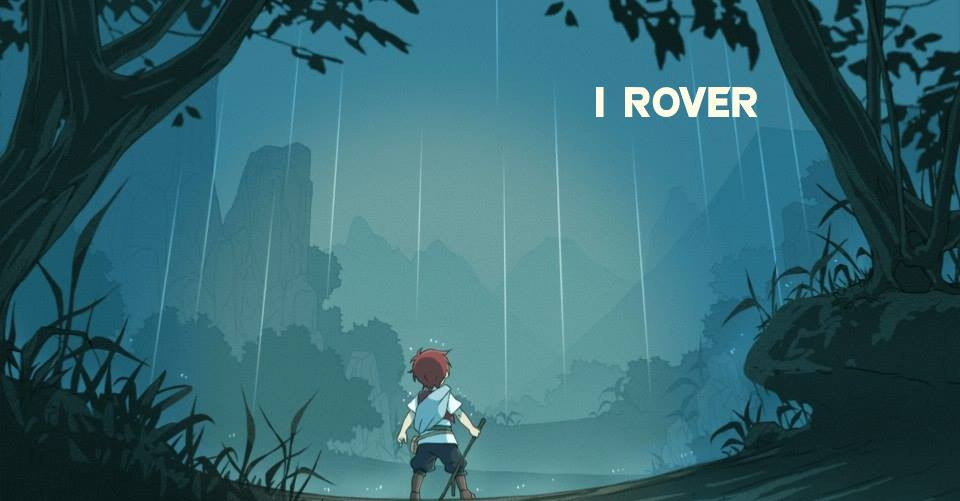
\includegraphics[width=350pt]{Illustration/proj_irover.jpg}
	\caption{iRover, l'histoire d'un héros qu'on appellait robot}
\end{figure}



\newpage


\renewcommand{\contentsname}{Sommaire} 
\tableofcontents

\newpage





\section{Manuel Documentation Technique}


\vspace{2cm}

Cette partie est dédiée aux développeurs et aux utilisateurs expérimenté ayant une culture informatique.
Les divers éléments de l'application y sont décrit de façon plus mathématique et logique.
Vous pouvez vous rapprocher de la doc Doxygen pour avoir encore plus de détails.

\subsection{Génération Doc Doxygen}

executer la commande pour générer le fichier de config

\vspace{0.5 cm}
\begin{DDbox}{\linewidth}
\begin{verbatim}
doxygen -g config_dox
\end{verbatim}
\end{DDbox}


modifier les champs suivants dans le fichier de config :

\vspace{0.3 cm}


\begin{DDbox}{\linewidth}
\begin{verbatim}


PROJECT_NAME           = "I-rover"

PROJECT_NUMBER         = 1.0

OUTPUT_LANGUAGE        = French
INPUT                  = CodeMain

FILE_PATTERNS          = *.hpp *.cpp


\end{verbatim}
\end{DDbox}


executer la commande :

\vspace{0.3 cm}

\begin{DDbox}{\linewidth}
\begin{verbatim}

doxygen config\_dox
\end{verbatim}
\end{DDbox}
\vspace{0.3 cm}

\newpage
\section{Les personnages}
Le jeu possède des personnages. Ceux-ci sont représentés par la classe personnage. Tous les personnages possèdent des attributs:
\begin{enumerate}
	\item positionX: La position du personnage sur l'axe x.
	\item positionY: La position du personnage sur l'axe y.
	\item arme: L'arme qui possède le personnage.
	\item armure: L'armure que possède le personnage.
	\item puissance: La puissance du personnage, déterminée à partir de son arme.
	\item robustesse: La robustesse du personnage, déterminée à partir de son armure.
	\item isActive: Pour savoir si le personnage est encore en vie.
	\item sprite: L'image du personnage dans le jeu.
	\item collision map: Un vecteur qui détermine les endroits où le personnage peut aller.
\end{enumerate}

Grâce à ces attributs, tous les personnages peuvent se déplacer d'une case grâce à la méthode deplacer(int x,int y). Les personnages peuvent aussi combattre d'autres personnages grâce à la méthode combattre(Personnage* personnage).

Le vainqueur d'un combat est déterminé par celui qui a la plus grande chance de gagner. Les deux adversaires tirent un nombre déterminé par l'algorithme suivant :

\begin{equation}
    random() \times puissance \times robustesse 
    \label{combat}
\end{equation}

Ainsi on compare ces deux nombres. Celui qui a le plus grand gagne le duel.

\subsection{Le robot, Rover}

Le robot, en plus d'hériter des propriétés des personnages, possède un attribut \emph{inventaire} qui représente le nombre de clefs qu'il possède.

L'objectif du robot est d'ouvrir tous les coffres de la carte et chaque coffre s'ouvre à l'aide d'une clef. Ainsi, le robot possède les méthodes \emph{ramasser
(Clef* clef)} ou \emph{ouvrir(Coffre* coffre)}.

Le robot se déplace d'une certaine manière, grâce à un algorithme de pathfinding\ref{pathfinding}.

\subsection{Les ennemis}

Un ennemi est un simple personnage qui a sa propre façon de se déplacer et de combattre. 
Un ennemi se déplace aléatoirement sur la carte, et continue tant que la partie n'est pas finie ou tant qu'il est encore en vie.

Lorsqu'un ennemi est à une case du robot, alors celui-ci affronte le robot.


\section{Les coffres}

Les coffres sont de simples objets qui possèdent les propriétés suivantes: 

\begin{enumerate}
	\item positionX: sa position sur l'axe x.
	\item positionY: sa position sur l'axe y. 
	\item ouvert: booléen qui permet de savoir si le coffre est ouvert ou fermé.
	\item sprite: l'image du coffre.
\end{enumerate}

Une fois le coffre ouvert, son paramètre ouvert passe à true et ne peut donc plus s'ouvrir.


\section{Les clef}

Les clefs ont les mêmes attributs que les coffres excepté pour l'attribut ouvert. Une fois la clef ramassée, celle-ci disparait de la carte et l'inventaire du robot augmente de 1.

\section{Les actuateurs}

Le robot, tout comme les ennemis possèdent deux sortes d'actuateurs: les armes et les armures.

Ces armes et armures déterminent la puissance et la robustesse de chaque personnage du jeu.

Plusieurs armes existent dans le jeu, un bazooka qui augmente fortemment la puissance du possesseur, des mines que le personnage laisse derrière lui régulièrement\ldots

Grâce à ces différents actuateurs, il est possible de choisir sa stratégie selon le nombre d'ennemis sur la carte, la forme de la carte\ldots

Toutes les armes héritent de la classes Arme et les armures de la classe Armure. Ainsi, i lest facile de créer de nouveaux types d'armes et armures.

\section{Les senseurs}

Le robot possède un scanner. Celui-ci permet de scanner une map et de savoir quels sont les endroits où il peut aller et les endroits qui lui sont inacessibles.

\newpage
\section{L'environnement}

Le terrain est représenté par la classe \textbf{Map}, qui contient les informations sur ce terrain (hauteur, largeur, taille des cases) et deux matrices contenant respectivement les types de cases de la carte, et la praticabilité de celles-ci. Cette dernière matrice est passée aux entités évoluant dans cette carte, pour connaître les cases passables ou non et adapter leurs algorithmes de recherche de chemin en conséquence.
Une carte se construit à partir d'un fichier au format \emph{.tmx}, un format de carte géré par le logiciel \textbf{Tiled}, un éditeur de cartes libre. Ce fichier est alors traîté comme un document DOM, grâce au module \emph{ClanXML} de la bibliothèque \emph{ClanLib 4.0}, pour en extraire les informations et les numéros des cases.
Pour gérer le dessin de la carte, la classe \textbf{Tileset} permet de représenter une feuille de textures consistant en une image regroupant toutes les textures des cases pouvant être dessinées. Ce tileset possède des métadonnées telles que le nombre de textures en lignes, colonnes, leur taille en pixels et l'espacement entre chacun dans l'image, métadonnées qui peut être récupérées également depuis le fichier de carte .tmx fourni. A partir d'un numéro de tile à une certaine position dans la carte, on peut alors déterminer quelle texture doit être dessinée à l'emplacement correspondant. 
La classe \textbf{mapDisplay} est pour l'instant la classe principale de l'application, où sont affichés la carte et tous les éléments interagissant avec. Tout l'affichage est géré par le module \emph{ClanDisplay} de la bibliothèque \emph{ClanLib 4.0}, qui dessine au milieu de la fenêtre toute la carte case par case conformément au Tileset fourni, ainsi que tous les personnages et les objets.

\section{La gestion des évênements}

La gestion des évênemments concerne toutes les actions que peuvent faire les personnages dans le jeu.

\subsection {Rencontre avec un ennemi} 

Lorsque le robot rencontre un ennemi, un combat se déclenche. Une des deux personnages en sort vainqueur, si le robot gagne alors la partie continue, sinon la partie s'arrête.

\subsection {Ouverture d'un coffre}

Lorsque le robot possède au moins une clef et qu'il se trouve à la même position qu'un coffre, alors il l'ouvre. Le statut ouvert du coffre passe donc à true.

\subsection {Ramasser une clef}

Lorsque le robot est à la même position qu'une clef, celui-ci la ramasse automatiquement. Son attribut inventaire est donc incrémenté de 1.



\section{IA}

\subsection{path finding}
Le code responsable du pathfinding est contenu dans \emph{astar} défininissant la classe \emph{Node} et la méthode \emph{pathFind()}. Grâce à cette méthode on obtient le plus court chemin entre un objet et un couple de coordonnées sur la carte. Le chemin est obtenu sous la forme d'une chaîne de caractères, chaque caractère étant 0, 1 ,2 ou 3 et correspondant à un mouvement à effectuer comme suit:
\begin{enumerate}
\item 0:Le personnage se déplace d'une case à droite
\item 1:Le personnage se déplace d'une case vers le bas
\item 2:Le personnage se déplace d'une case à gauche
\item 3:Le personnage se déplace d'une case vers le haut
\end{enumerate}

La fonction \emph{goTo()} lit cette chaîne de caractères et réalise les différents mouvements à l'aide de la fonction \emph{deplacer()};
\subsection{découverte de la carte}
L'exploration et le pathfinding sont testés dans la classe \emph{MapDisplayTestPathfinding}, qui est une modification de la classe \emph{MapDisplay}.
\subsubsection{Exploration du robot}
Le robot a accès aux coordonnées de l'ensemble des clefs et des coffres. Si il ne possède pas de clefs, il cherche la clef la plus proche avec la fonction \emph{findNearestKey()} et s'y dirige.
Ensuite il cherche le coffre le plus proche avec la fonction \emph{findNearestChest()} et s'y dirige.
La clef étant normalement détruite après avoir ouvert le coffre, le robot peut effectuer ces actions en boucle.

\subsubsection{Exploration des ennemis}
Un ennemi reçoit des coordonnées aléatoires(contenues dans la carte) et s'y déplace avec la fonction \emph{goTo()}.



\end{document}

